\section{Risk Parity Portfolios}

\begin{frame}[t]\frametitle{Risk Measures}\bigskip
	\begin{definition}[5.1]
		A portfolio with $n$ assets, $A_1, A_2, \dots, A_n$, is a vector $x^\top = (x_1, x_2, \dots, x_n)\in \R^n$, each coordinate $x_i$ being the weight of the capital invested in asset $A_i$.
	\end{definition}

	\bigskip

	One way to measure the risk of portfolio is by its volatility, i.e, the standard deviation of its daily returns.

	\bigskip

	If we denote by $\mu$ and $\Sigma$ the vector of expected returns and the covariance matrix of asset returns respectively, we deduce that the expected return of portfolio $x$ equals:
	\begin{equation}
		\mu(x) = x^\top \mu.
	\end{equation}
	Its variance is given by:
	\begin{equation}
		\sigma^2(x) = x^\top \Sigma x.
	\end{equation}
\end{frame}

\begin{frame}[t]\frametitle{Minimum Variance Portfolio (MVP)}\bigskip
	The \textcolor{purple}{minimum variance portfolio} (MVP) of Markowitz\footfullcite{Markowitz1952}, consists of minimize variance with fully invested capital, achieved by solving the problem:
	\begin{eqnarray}\label{eq:MVP}
		\min_{x} \,\big\{x^\top \Sigma x\big\}, \\
		\mbox{s.t. }\left\{
		\begin{aligned}
			\mathbf{1}^\top x=1. \\
		\end{aligned}
		\right.\nonumber
	\end{eqnarray}
	where $\textbf{1}^\top =(1,1,\dots,1)$.
\end{frame}

\begin{frame}[t]\frametitle{Risk Parity Portfolio (RPP)}\bigskip
	Let $x^\top=(x_1,x_2,\dots,x_n)$ be a portfolio with $n$ assets and $\mathcal{R}(x)$ be a differentiable, homogeneous risk measure of $x$. We have
	\begin{equation}
		\mathcal{R}(x)=\frac{d}{d\lambda}\mathcal{R}(\lambda x)=\sum_{i=1}^n x_i \frac{\partial \mathcal{R} (x)}{\partial x_i}.
	\end{equation}
	We define the risk contribution of asset $i$  as
	\begin{equation}
		\mathcal{RC}_i(x)= x_i \frac{\partial \mathcal{R}(x)}{\partial x_i}.
	\end{equation}
	Therefore, the risk may be written as follows
	\begin{equation}
		\mathcal{R}(x)=\sum_{i=1}^n \mathcal{RC}_i(x)
	\end{equation}
	which is known as \textbf{Euler's Allocation Principle}.

\end{frame}

\begin{frame}[t]\frametitle{Risk Parity Portfolio (RPP)}\bigskip
	It may be interesting for the investor to choose different risk levels for different assets. In this case the investor choose the percentage of risk, $b_i$, that each asset should have in the portfolio, that is,
	\begin{equation}\label{eq:RBP}
		\mathcal{RC}_i(x)=b_i\mathcal{R}(x),
	\end{equation}
	$b_i\geq 0$ for all $i$, and
	${\bf 1}^\top b =1$, with $b^\top=(b_1, b_2, \dots, b_n)$. A portfolio distribution based on equation \eqref{eq:RBP} is called a \textcolor{purple}{\textit{risk budgeting portfolio}} (RBP). When $b_i=1/n$, for all $i$, the distribution is called \textcolor{purple}{\textit{risk parity portfolio}} (RPP) or \textcolor{purple}{\textit{equal risk portfolio}} (ERP).

	In general, find the risk budgeting portfolio consists in solving the following non-linear system
	\begin{eqnarray}
		\mathcal{RC}_i(x)=b_i\mathcal{R}(x), \nonumber\\
		\mbox{s.t. }\left\{
		\begin{aligned}
			b_i \geq 0,        \\
			x_i \geq 0,        \\
			{\bf 1}^\top b =1, \\
			{\bf 1}^\top x =1.
		\end{aligned}
		\right.
	\end{eqnarray}
\end{frame}

\begin{frame}[t]\frametitle{Risk Parity Portfolio(RPP)}\bigskip
	Kaya and Lee \footfullcite{KayaLee2012} show that, in the Gaussian case, the risk budgeting portfolio may be found solving the optimization problem
	\begin{eqnarray}
		\min_{x> \textbf{0}}\, \{-b^\top \ln(x)\}; \label{eq:RPP}\nonumber\\
		\mbox{s.t. }\left\{ 
		\begin{aligned}
			\sigma^2(x)\leq \sigma_0, \\
			{\bf 1}^\top x =1,
		\end{aligned}
		\right.
	\end{eqnarray}
	$\sigma_0$ being a volatility target.
\end{frame}

\begin{frame}[t]\frametitle{Backtest Study}\bigskip
	We present an application for Algorithm~InexProj-SGM, a backtest study of a portfolio build with the 10 biggest companies on the brazilian market:

	Ambev S.A. (ABEV3), B3 S.A. (B3SA3), Banco do Brasil S.A. (BBAS3), Banco Bradesco S.A. (BBDC4), Itaúsa S.A. (ITSA3), Itaú Unibanco S.A. (ITUB4), Lojas Renner S.A. (LREN3), Petróleo Brasileiro S.A (PETR4), Vale S.A. (VALE3) and WEG S.A. (WEGE3).

	We did a backtest, building 2 portfolios with monthly rebalance:
	\begin{itemize}
		\item One was the minimum variance portfolio (MVP),
		\item the other the risk parity portfolio (RPP).
	\end{itemize}

	Data pertaining to the period between January 2016  and June 2022, was taken from Yahoo Finance (\url{http://finance.yahoo.com}). For rebalancing, the volatilities were calculated using data from the previous 12 months. 2016 year data was used only for past volatilities calculations.
\end{frame}

\begin{frame}[t]\frametitle{}
	\begin{figure}[H]
		\begin{adjustwidth}{1cm}{1cm}
			\begin{subfigmatrix}{2}
				\subfigure[Weigths]{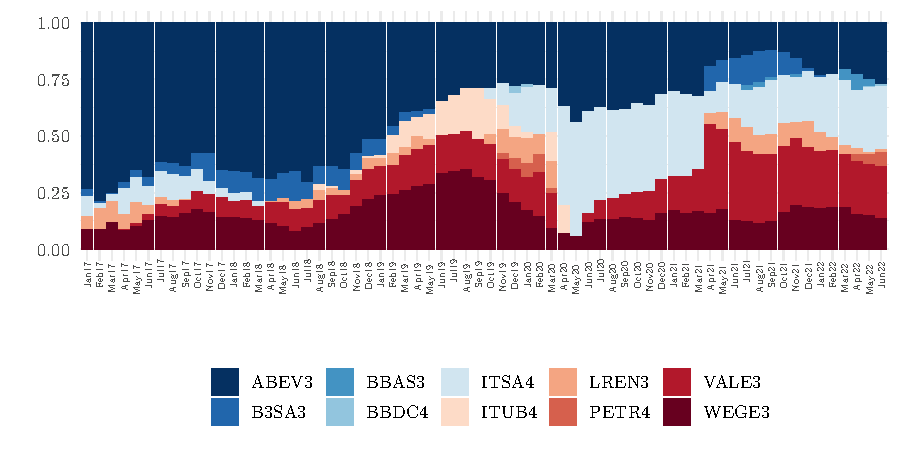
\includegraphics{../figures/totalWeigthMVP.pdf}}
				\subfigure[Risks]{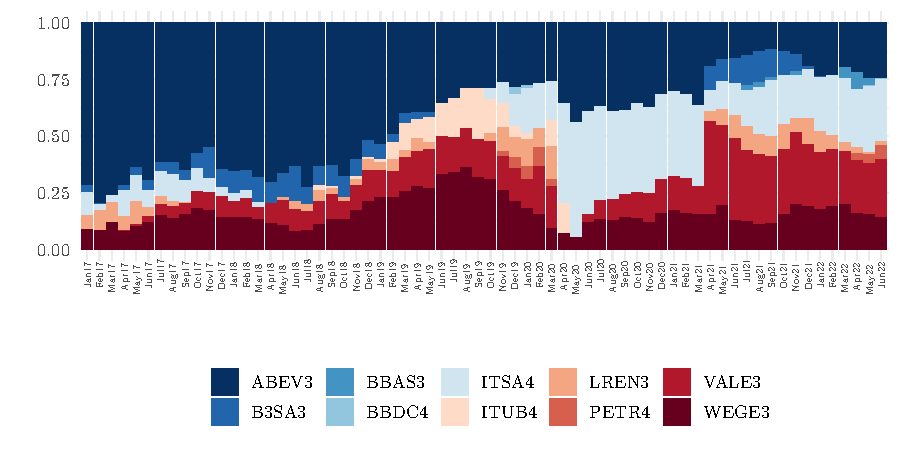
\includegraphics{../figures/totalRiskMVP.pdf}}
			\end{subfigmatrix}
			\caption{Monthly distribution of MVP.}
			\label{fig:totalRiskMVP}
		\end{adjustwidth}
	\end{figure}


	\begin{figure}[H]
		\begin{adjustwidth}{1cm}{1cm}
			\begin{subfigmatrix}{2}
				\subfigure[Weigths]{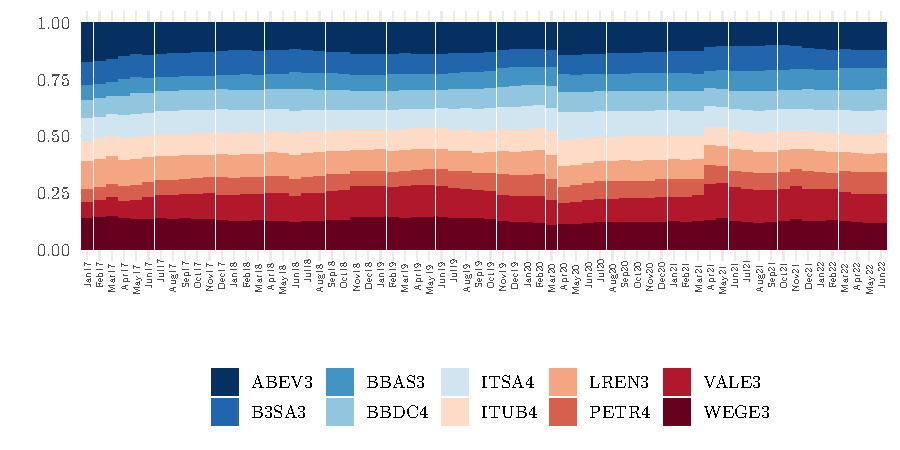
\includegraphics{../figures/totalWeigthRPP.pdf}}
				\subfigure[Risks]{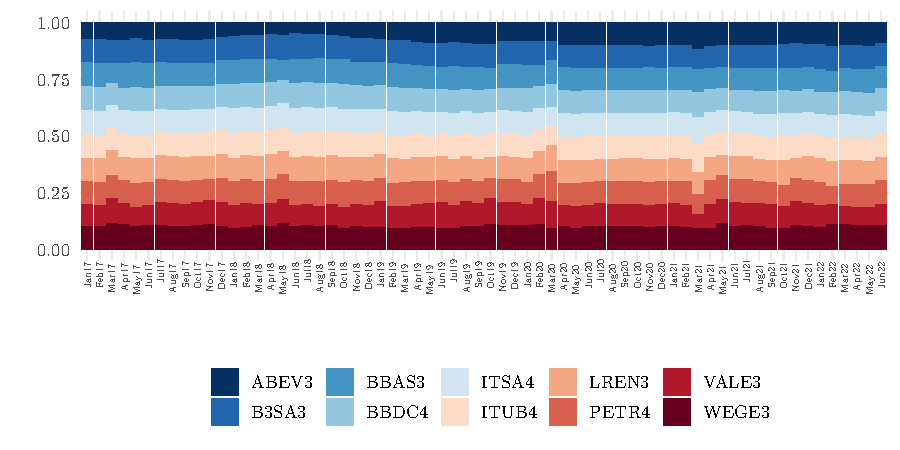
\includegraphics{../figures/totalRiskRPP.pdf}}
			\end{subfigmatrix}
			\caption{Monthly distribution of RPP.}
			\label{fig:totalRiskPPP}
		\end{adjustwidth}
	\end{figure}
\end{frame}

\begin{frame}[t]\frametitle{}\bigskip

	\begin{figure}[H]
		\centering
		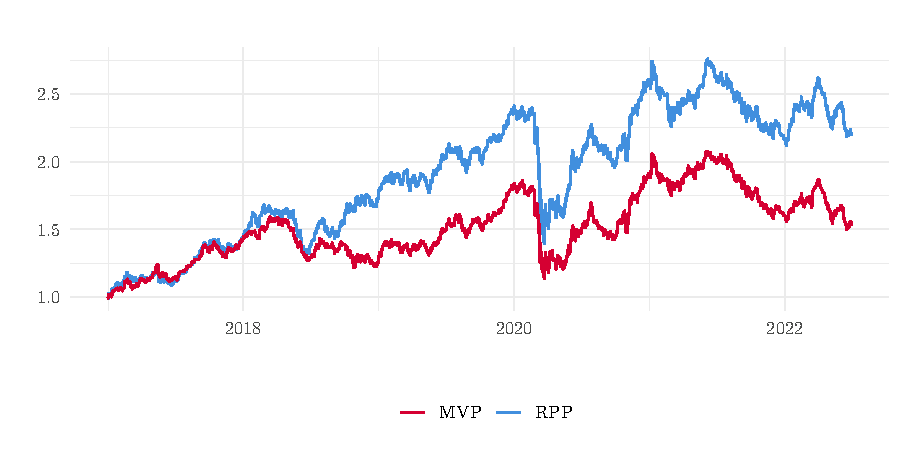
\includegraphics[width=0.7\linewidth]{../figures/retornoRPPMVP.pdf}
		\caption{MVP and RPP accumulated returns: January 2017 $-$ June 2022.}
		\label{fig:retornoRPPMVP}
	\end{figure}


	\begin{table}[!htb]
    \centering
      \begingroup
      \fontsize{9}{9}
      \selectfont 
\begin{tabular}{>{}lrr}
\toprule
  & MVP & RPP\\
\midrule
\textbf{Annualized Return} & 0.0785 & 0.1505\\
\textbf{Annualized Std Dev} & 0.2419 & 0.2637\\
\textbf{Annualized Sharpe (Rf=0\%)} & 0.3246 & 0.5708\\
\bottomrule
\end{tabular} \caption{Annualized returns: January 2017 - June 2022.}
      \label{tab:RPP}  % LEMBRE-SE DE MUDAR O LABEL
      \endgroup{}
      \end{table}


\end{frame}

\begin{frame}[t]\frametitle{}\bigskip

	\begin{figure}[H]
		%\begin{adjustwidth}{2.2cm}{2.2cm}
		\begin{subfigmatrix}{2}
			\subfigure[January 2017 $-$ December 2019.]{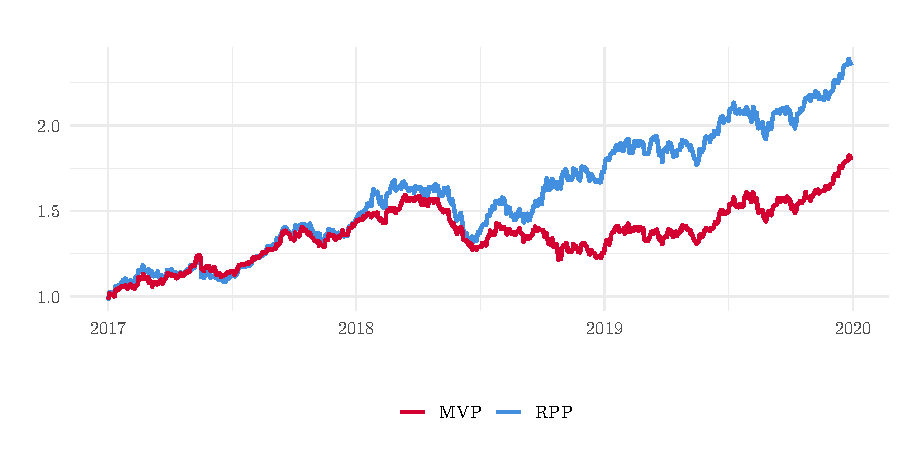
\includegraphics{../figures/retornoRPPMVP1.pdf}}
			\subfigure[January 2020 $-$ June 2022.]{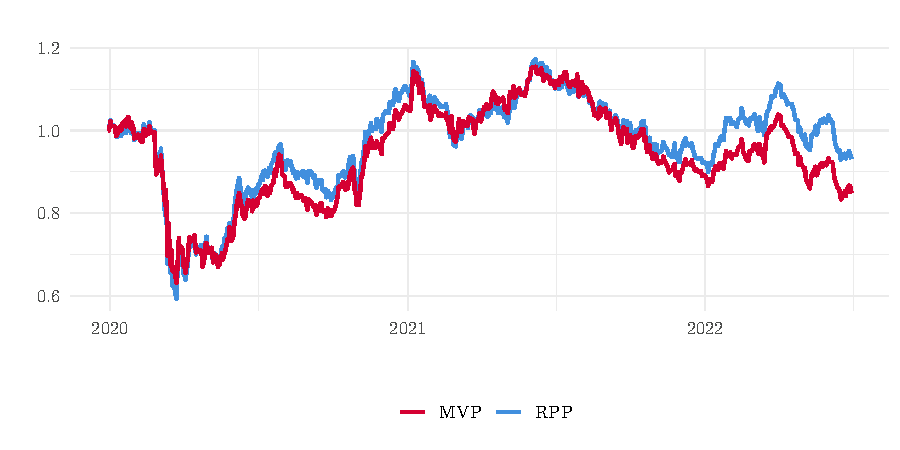
\includegraphics{../figures/retornoRPPMVP2.pdf}}
		\end{subfigmatrix}
		\caption{MVP and RPP accumulated returns.}
		%	\label{fig:retornoRPPMVP12}
		%\end{adjustwidth}
	\end{figure}


	\begin{table}[!htb]
		% \caption{Global caption}
		\begin{minipage}{.5\linewidth}
			\begin{table}[!htb]
				\centering
				\begingroup
				\fontsize{7}{7}
				\selectfont
				\begin{tabular}{>{}lrr}
					\toprule
					                                    & MVP    & RPP    \\
					\midrule
					\textbf{Annualized Return}          & 0.2107 & 0.3212 \\
					\textbf{Annualized Std Dev}         & 0.1744 & 0.2027 \\
					\textbf{Annualized Sharpe (Rf=0\%)} & 1.2087 & 1.5851 \\
					\bottomrule
				\end{tabular} \caption{January 2017 - December 2019.}
				%	\label{tab:RPP1}  % LEMBRE-SE DE MUDAR O LABEL
				\endgroup{}
			\end{table}
		\end{minipage}%
		\begin{minipage}{.5\linewidth}
			\begin{table}[!htb]
				\centering
				\begingroup
				\fontsize{7}{7}
				\selectfont
				\begin{tabular}{>{}lrr}
					\toprule
					                                    & MVP     & RPP     \\
					\midrule
					\textbf{Annualized Return}          & -0.0631 & -0.0278 \\
					\textbf{Annualized Std Dev}         & 0.3046  & 0.3227  \\
					\textbf{Annualized Sharpe (Rf=0\%)} & -0.2070 & -0.0860 \\
					\bottomrule
				\end{tabular}
				\caption{January 2020 - June 2022.}
				%	\label{tab:RPP2}  % LEMBRE-SE DE MUDAR O LABEL
				\endgroup{}
			\end{table}
		\end{minipage}
	\end{table}
\end{frame}